\documentclass[letterpaper, conference]{IEEEtran}

\usepackage{amsmath}
\DeclareMathOperator*{\argmax}{argmax}

\usepackage{pgfplots}
\pgfplotsset{compat=1.5.1}

\usepackage{titlesec}
\titlespacing*{\subsection}{0pt}{1.1\baselineskip}{\baselineskip}
\setlength{\parindent}{2em}
\setlength{\parskip}{0.7em}

\usepackage{url}

\begin{document}

\title{ML Midterm Report}

\author{
  \IEEEauthorblockN{Alvaro Faundez}
  \IEEEauthorblockA{
    \textit{Master in Data Science, first year}\\
    \textit{CUNY Graduate Center}\\
    \textit{alvaro@faundez.net}
  }
}

\maketitle

\begin{abstract}

The midterm project consists of the implementation of a discrete bayesian classifier. The subroutines include a dataset generator, training based on, and optimization of class conditional probabilities to maximize the expected gain. This report describes the steps that generate pseudo-random probabilities distributions, the dataset generation, the calculation of the Bayes decision rule, confusion matrix, and expected gain. The experimental results show that a 100\% expected gain is achievable in a few optimizations iterations.

\end{abstract}

\section{Introduction}

The Bayesian classifier is a popular predictive classifier broadly used in Machine Learning. Given a set of classes

\begin{equation} \label{classes}
C = \{c_1, ..., c_K\}
\end{equation}

and a measurement space

\begin{equation} \label{dimensions}
D = \times_{n=1}^{N}L_n
\end{equation}

the objective is to assign a class $c \in C$ for a specific measurement $d \in D$.

The critical step for the building of the Bayes decision rule is to calculate the posterior probability for a $d$:

\begin{equation} \label{eq:bayes}
P(c \mid d) \propto P(d \mid c) P(c)
\end{equation}

and use the economic gain matrix

\begin{equation}
  e =
  \begin{pmatrix}
    e(c_1,c_1) & \cdots & e(c_1,c_K) \\
      \vdots   & \ddots &    \vdots   \\
    e(c_K,c_1) & \cdots & c(c_K,c_K) 
  \end{pmatrix}
\end{equation}

to determine the $c_k$ with the highest economic gain

\begin{equation}
  \argmax_{c_k \in C} \sum_{j = 1}^{K} e(c_j, c_k)P(c_j, d)
\end{equation}

Then, the Bayes decision rule is defined as:

\begin{equation}
  f_d(c_m) = \left\{
  \begin{array}{lr}
  1 & m = k\\
  0 & m \neq k
  \end{array}\right\}
\end{equation}

The expected gain $E$, using an economic gain matrix $e$ is define as follows:

\begin{equation}
  E[e, f] = \sum_{c \in C} \sum_{d \in D}f_d(c)e(c, c)P(c \mid d)
\end{equation}

This report details the implementation of a Bayesian classifier from scratch in the Ruby language, without any external scientific library. The subroutines include

\begin{itemize}

  \item Class and measurement dimensions definitions, including pseudo-random probabilities and cumulative distribution functions

  \item Space definition, calculating linear addresses, class conditional probabilities
 
  \item Data set definition, in charge of the prior probabilities, the Bayes decision rule, the confusion matrix, and the expected gain

\end{itemize}

These definitions provide tools to train and test using multiple pseudo-random generated datasets. The random seed is configurable by the user to get the same result in any iteration.

The classifier can be optimized after the training, maximizing the expected gain, modifying the class conditional probabilities using, and arbitrary $\Delta$.

The experimental results achieve a 100\% expecting gain after only a couple of iterations.

\section{Technical}

\subsection{Requirements}

To run the code is necessary a Unix environment with Ruby 2.6+. The code is available on GitHub at \url{https://github.com/afaundez/ml-midterm}.

To test the command and check the available options run

\begin{verbatim}
  $ ./midterm --help
\end{verbatim}

\subsection{options}

For the purpose of testing, the following parameters are available for configuration

\begin{itemize}
    \item-s, --seed [INT]                 Pseudo-random seed, an integer. Default: nil
    \item-c, --classes [INT]              Class cardinality, an integer. Default 2
    \item-m, --measurements [INT]         Measurements size, an integer. Default 5
    \item    --measurement-min-cardinality [INT]
                                     Measurement Min Cardinality, an integer. Default 3
    \item    --measurement-max-cardinality [INT]
                                     Measurement Max Cardinality, an integer. Default 6
    \item    --sample-size [INT]          Sample size, an integer. Default to 10 times the  space addresses size.
    \item-i, --iterations [INT]           Iterations, an integer. Default 2
    \item-d, --delta [FLOAT]              Delta for conditionals improvement, a float. Default: 0.01
    \item    --no-overlap                 Generate classes based on measurements
    \item    --uniform                    Use uniform distribution on all dimensions
\end{itemize}

\subsection{Runtime}

\subsubsection{Build}

During the build, three significant abstractions are used: Dimension, Space, and DataSet.

The Dimension abstraction is meant to store the cardinality, probabilities distribution function, and cumulative distribution function of a single measurement or class. A dimension does not store values, but it can be used to generate random values using the distribution functions. A Dimension is defined by:

\begin{itemize}
  \item size
  \item pdf, generated based on the size
  \item cdf, generate based on the pdf
  \item distribution, whether to use random or uniform distribution
\end{itemize}

The Space abstraction stores the single class dimension \ref{classes}, the collection of measurements dimensions \ref{dimensions}, and the class conditional probabilities. Since the Space knows all the dimensions specifications, it is in charge of translating and measurement into a linear address and vice-versa. A Space is defined by:

\begin{itemize}
\item class\_dimension, a Dimension instance
\item measurements\_dimensions, a collection of Dimension instances
\item likelihoods, random pdfs
\end{itemize}

The DataSet abstraction is in charge of generating and store measurement values and the associated class, all bounded to a specific space. Since it has access to the data and space, it is in charge of the training and improving the class conditional probabilities, determining the Bayes Decision Rule, generating the Confusion Matrix, and calculating the Expected Gain. It is relevant that at creating the measurements, the prior class probabilities are calculated and stored in the DataSet. A DataSet is defined by:
    
\begin{itemize}
\item size
\item space, a Space instance
\item samples, a collection of collections of measurements
\item class\_outcomes, counter of classes for prior class probabilities calculation
\item overlap, whether to assign classes with overlap
\end{itemize}

The Economic Gain Matrix is generated in this step. Even though it is a method, currently, the only matrix available is the identity matrix.

\subsubsection{Training}

Once a set of DataSet is created, the test DataSet is picked and left isolated, and the rest is used as train DataSet.

The training process consists of two steps: using an economic gain matrix as input, outputs the Bayes decision rule, and the expected gain. Then, using the Bayes decision rule, it generates the confusion matrix.


At the end of this process, the Space associated with the DataSet will store the measurement conditional probabilities $P(c \mid d)$ targeted in \ref{eq:bayes}.

\subsection{Optimization}

Now that the space is trained and the measurement conditional probabilities have been processed, using the delta as input, the dataset can improve the class conditional probabilities using the test DataSet. For each mismatched classification, the corresponding class conditional probability is incremented by the delta input, and the measurement probabilities are normalized to 1. This process yields an updated Space and accuracy obtained.

\section{Experimental Results}

Even though it is not a strict test, it is good to do a sanity check with a dummy case: one feature, one value measurement. It is expected to have an expected gain of 1.0 and an accuracy of 1.0.

Running

\begin{verbatim}
  bin/midterm --classes 1 --measurements 1
\end{verbatim}

yields, as expected,

\begin{verbatim}
Economic Gain Matrix
+---+
| 1 |
+---+

Train 0.
  Expected Gain: 1.0
  Confusion Matrix Trace: 1.0
  Accuracy: 1.0
Confusion Matrix
+-----+
| 1.0 |
+-----+

Test
  Expected Gain: 1.0
  Confusion Matrix Trace: 1.0
  Accuracy: 1.0
\end{verbatim}


The next step is to check the results using. Let us use two classes, five values measurements, and ten training sets, and start setting the seed number in order to have replicable experiments.

\subsection{First results}

\begin{verbatim}
  bin/midterm --classes 2 --measurements 5 \
    --iterations 10 --seed 1234
\end{verbatim}

The expected gain and accuracy do not seem to be correct

\vspace{1cm}
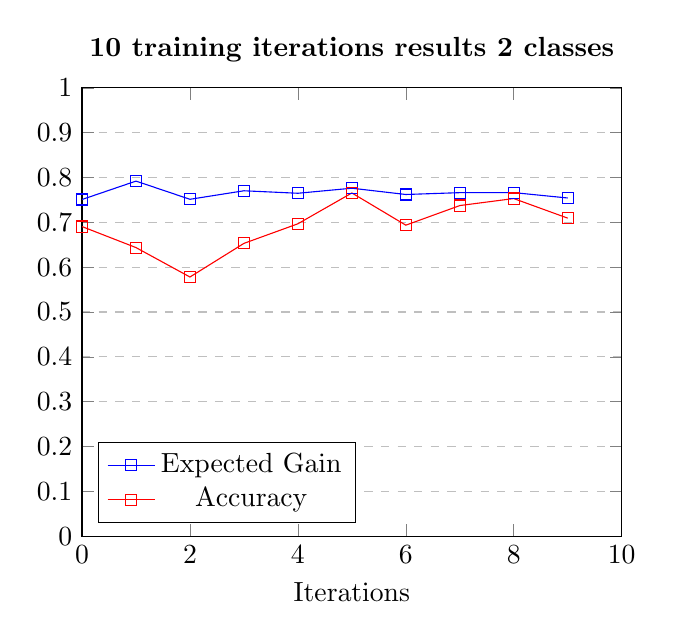
\begin{tikzpicture}
\begin{axis}[
    title=\textbf{10 training iterations results 2 classes},
    xlabel={Iterations},
    xmin=0, xmax=10,
    ymin=0.0, ymax=1,
    xtick={0,2,4,6,8,10},
    ytick={0.0,0.1,0.2,0.3,0.4,0.5,0.6,0.7,0.8,0.9,1.0},
    legend pos=south west,
    ymajorgrids=true,
    grid style=dashed,
]

\addplot[color=blue, mark=square]
  coordinates {
    (0, 0.7510161862543873)
    (1, 0.7920788037709293)
    (2, 0.7514642101011255)
    (3, 0.7704808259436531)
    (4, 0.7649375191939426)
    (5, 0.776186768335381)
    (6, 0.7621880262547054)
    (7, 0.7662678293114988)
    (8, 0.766369437713792)
    (9, 0.7543597171481017)
  };
  \addlegendentry{Expected Gain}

\addplot[color=red, mark=square]
  coordinates {
    (0, 0.690625)
    (1, 0.64375)
    (2, 0.578125)
    (3, 0.653125)
    (4, 0.696875)
    (5, 0.765625)
    (6, 0.69375)
    (7, 0.7375)
    (8, 0.753125)
    (9, 0.709375)
  };
  \addlegendentry{Accuracy}
    
\end{axis}
\end{tikzpicture}
\vspace{1cm}

Incrementing the training iterations to 100 does not make real improvements; it keeps going up and down.

\vspace{1cm}
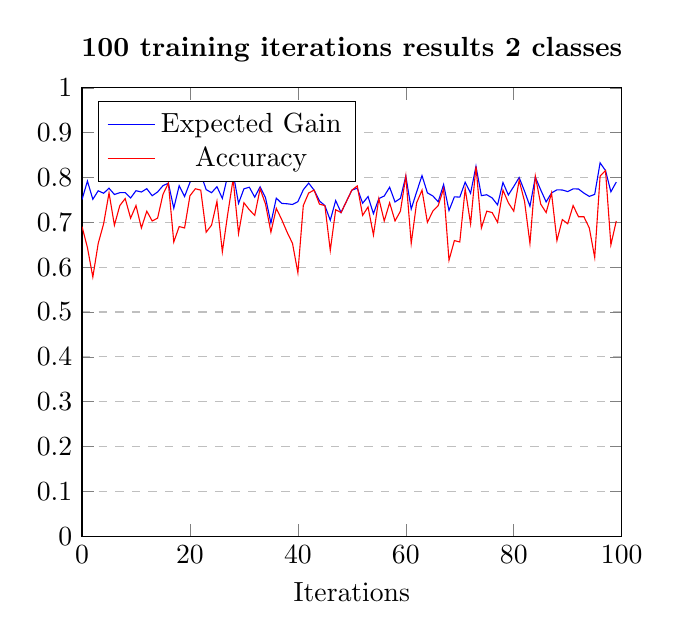
\begin{tikzpicture}
\begin{axis}[
    title=\textbf{100 training iterations results 2 classes},
    xlabel={Iterations},
    xmin=0, xmax=100,
    ymin=0.0, ymax=1,
    xtick={0,20,40,60,80,100},
    ytick={0.0,0.1,0.2,0.3,0.4,0.5,0.6,0.7,0.8,0.9,1.0},
    legend pos=north west,
    ymajorgrids=true,
    grid style=dashed,
]

\addplot[color=blue, mark=dot]
  coordinates {
    (0,0.7510161862543873)
    (1,0.7920788037709293)
    (2,0.7514642101011255)
    (3,0.7704808259436531)
    (4,0.7649375191939426)
    (5,0.776186768335381)
    (6,0.7621880262547054)
    (7,0.7662678293114988)
    (8,0.766369437713792)
    (9,0.7543597171481017)
    (10,0.7706252669070704)
    (11,0.7677486854798666)
    (12,0.775107105978118)
    (13,0.7594228327421679)
    (14,0.7677920561126736)
    (15,0.7818246469717948)
    (16,0.7875)
    (17,0.7315601669135878)
    (18,0.7818142947781787)
    (19,0.7576822006522522)
    (20,0.7891927339222548)
    (21,0.8080828660665679)
    (22,0.808291232475898)
    (23,0.7731074214835443)
    (24,0.7661685725706955)
    (25,0.7795960922267542)
    (26,0.7534918836091349)
    (27,0.804382002795244)
    (28,0.8101265043180191)
    (29,0.7423507571843759)
    (30,0.7748956360257283)
    (31,0.7783760561971604)
    (32,0.7563671770160953)
    (33,0.7794164114191516)
    (34,0.7548549972084373)
    (35,0.6985936048835456)
    (36,0.7540787594223081)
    (37,0.7423220518369233)
    (38,0.7414790690273345)
    (39,0.7399310419882174)
    (40,0.7461861573924471)
    (41,0.7726672440595368)
    (42,0.7875930169360047)
    (43,0.771875)
    (44,0.7478136145141515)
    (45,0.7375)
    (46,0.7046454035552939)
    (47,0.7485827502762095)
    (48,0.721875)
    (49,0.746875)
    (50,0.7718750000000001)
    (51,0.7762767921268567)
    (52,0.742722038380545)
    (53,0.7576363133297808)
    (54,0.719379621732634)
    (55,0.753125)
    (56,0.7587679107898118)
    (57,0.7784285726715959)
    (58,0.7454963471675674)
    (59,0.7535354049383377)
    (60,0.8031249999999999)
    (61,0.7296744616178817)
    (62,0.7679177662206217)
    (63,0.8042096987034367)
    (64,0.7658365604343714)
    (65,0.7589832786098533)
    (66,0.7459872520612136)
    (67,0.7844529837554968)
    (68,0.7264501536949466)
    (69,0.7569805135737274)
    (70,0.7562980808006607)
    (71,0.7897104955862423)
    (72,0.7650199909263249)
    (73,0.825)
    (74,0.7596274552431364)
    (75,0.7615740117441012)
    (76,0.7545261883433753)
    (77,0.7390097447410758)
    (78,0.7888259823660361)
    (79,0.7611479809409623)
    (80,0.7800389919957694)
    (81,0.8000670614704873)
    (82,0.7695309172984911)
    (83,0.7358039227270565)
    (84,0.8009030565080281)
    (85,0.7723536586165068)
    (86,0.7456604882424223)
    (87,0.765625)
    (88,0.7726276557725134)
    (89,0.7722226522650084)
    (90,0.7686710071464256)
    (91,0.7747661534177785)
    (92,0.7744289026320158)
    (93,0.7652564770408778)
    (94,0.7579334212203201)
    (95,0.7624714461070612)
    (96,0.8327829938086287)
    (97,0.8156250000000002)
    (98,0.7682514790928694)
    (99,0.7899015704803447)
  };
  \addlegendentry{Expected Gain}

\addplot[color=red]
  coordinates {
    (0,0.690625)
    (1,0.64375)
    (2,0.578125)
    (3,0.653125)
    (4,0.696875)
    (5,0.765625)
    (6,0.69375)
    (7,0.7375)
    (8,0.753125)
    (9,0.709375)
    (10,0.7375)
    (11,0.6875)
    (12,0.725)
    (13,0.703125)
    (14,0.709375)
    (15,0.7625)
    (16,0.7875)
    (17,0.65625)
    (18,0.690625)
    (19,0.6875)
    (20,0.759375)
    (21,0.775)
    (22,0.771875)
    (23,0.678125)
    (24,0.69375)
    (25,0.746875)
    (26,0.634375)
    (27,0.71875)
    (28,0.796875)
    (29,0.675)
    (30,0.74375)
    (31,0.728125)
    (32,0.715625)
    (33,0.775)
    (34,0.740625)
    (35,0.678125)
    (36,0.73125)
    (37,0.70625)
    (38,0.678125)
    (39,0.653125)
    (40,0.5875)
    (41,0.7375)
    (42,0.765625)
    (43,0.771875)
    (44,0.740625)
    (45,0.7375)
    (46,0.6375)
    (47,0.728125)
    (48,0.721875)
    (49,0.746875)
    (50,0.771875)
    (51,0.78125)
    (52,0.715625)
    (53,0.734375)
    (54,0.671875)
    (55,0.753125)
    (56,0.703125)
    (57,0.74375)
    (58,0.703125)
    (59,0.725)
    (60,0.803125)
    (61,0.653125)
    (62,0.74375)
    (63,0.771875)
    (64,0.7)
    (65,0.725)
    (66,0.7375)
    (67,0.775)
    (68,0.615625)
    (69,0.659375)
    (70,0.65625)
    (71,0.775)
    (72,0.696875)
    (73,0.825)
    (74,0.6875)
    (75,0.725)
    (76,0.721875)
    (77,0.7)
    (78,0.771875)
    (79,0.74375)
    (80,0.725)
    (81,0.79375)
    (82,0.746875)
    (83,0.653125)
    (84,0.803125)
    (85,0.740625)
    (86,0.721875)
    (87,0.765625)
    (88,0.659375)
    (89,0.70625)
    (90,0.696875)
    (91,0.7375)
    (92,0.7125)
    (93,0.7125)
    (94,0.6875)
    (95,0.621875)
    (96,0.803125)
    (97,0.815625)
    (98,0.65)
    (99,0.703125)
  };
  \addlegendentry{Accuracy}
    
\end{axis}
\end{tikzpicture}
\vspace{1cm}

To identify the reason of these results, two options were added to the application, one to control the overlap in the class assignment to a measurement and how the probability distribution is generated.

\subsection{Probability distributions}

Since the method used to generate the probability distribution function for a dimension does not generate even probabilities for each value in the dimension, a parameter $--uniform$ was added to revert this and generate uniform distribution for the classes and measurement. The hypothesis was that by generating numbers evenly, the results would easier to understand.

Now, repeating the previous commands with the new parameter:

\begin{verbatim}
  bin/midterm --classes 2 --measurements 5 \
    --iterations 10 --seed 1234 \
    --uniform
\end{verbatim}

\vspace{1cm}
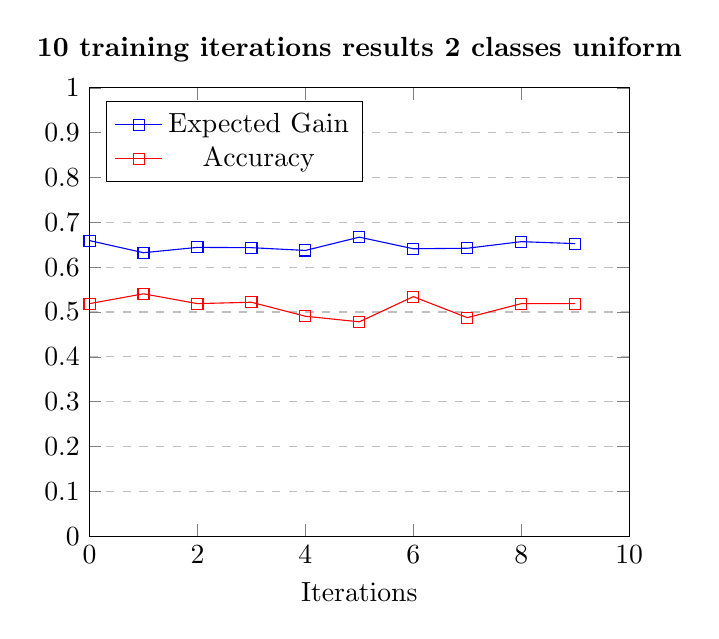
\begin{tikzpicture}
\begin{axis}[
    title=\textbf{10 training iterations results 2 classes uniform},
    xlabel={Iterations},
    xmin=0, xmax=10,
    ymin=0.0, ymax=1,
    xtick={0,2,4,6,8,10},
    ytick={0.0,0.1,0.2,0.3,0.4,0.5,0.6,0.7,0.8,0.9,1.0},
    legend pos=north west,
    ymajorgrids=true,
    grid style=dashed,
]

\addplot[color=blue, mark=square]
  coordinates {
    (0,0.6593504287948415)
    (1,0.6322952653288357)
    (2,0.6442318074145162)
    (3,0.643532034044156)
    (4,0.6374052549173173)
    (5,0.6670332218794528)
    (6,0.641154535217185)
    (7,0.6422862876918007)
    (8,0.6569850006437995)
    (9,0.6526304654809094)
  };
  \addlegendentry{Expected Gain}

\addplot[color=red, mark=square]
  coordinates {
    (0,0.51875)
    (1,0.540625)
    (2,0.51875)
    (3,0.521875)
    (4,0.490625)
    (5,0.478125)
    (6,0.534375)
    (7,0.4875)
    (8,0.51875)
    (9,0.51875)
  };
  \addlegendentry{Accuracy}
    
\end{axis}
\end{tikzpicture}
\vspace{1cm}

The expected gain does not seem to be improving, but the accuracy is set around $0.5$. It could be a sign that accuracy is bouncing between that particular number because now each class has the same probability of being assign to a measurement. Using 100 training iterations, the result is similar.

\vspace{1cm}
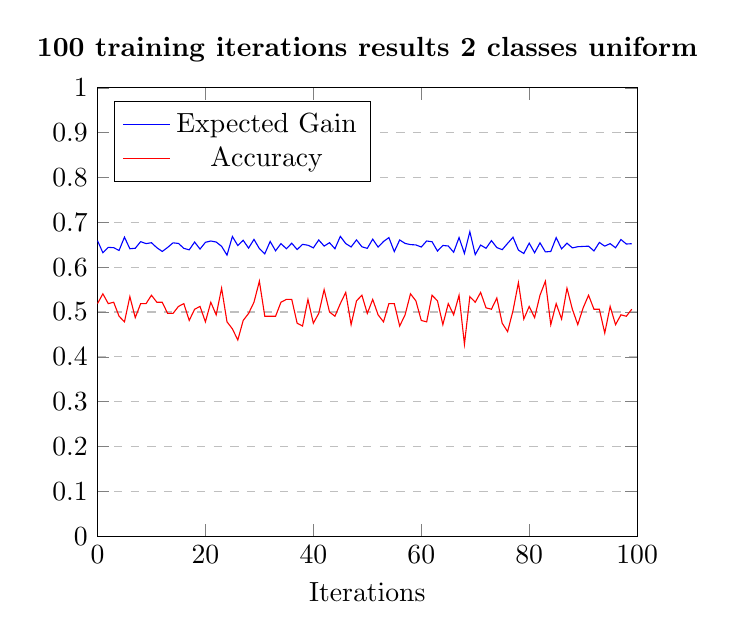
\begin{tikzpicture}
\begin{axis}[
    title=\textbf{100 training iterations results 2 classes uniform},
    xlabel={Iterations},
    xmin=0, xmax=100,
    ymin=0.0, ymax=1,
    xtick={0,20,40,60,80,100},
    ytick={0.0,0.1,0.2,0.3,0.4,0.5,0.6,0.7,0.8,0.9,1.0},
    legend pos=north west,
    ymajorgrids=true,
    grid style=dashed,
]

\addplot[color=blue, mark=dot]
  coordinates {
    (0,0.6593504287948415)
    (1,0.6322952653288357)
    (2,0.6442318074145162)
    (3,0.643532034044156)
    (4,0.6374052549173173)
    (5,0.6670332218794528)
    (6,0.641154535217185)
    (7,0.6422862876918007)
    (8,0.6569850006437995)
    (9,0.6526304654809094)
    (10,0.6546187941166898)
    (11,0.643475265753768)
    (12,0.6351244529764057)
    (13,0.6440720167792894)
    (14,0.6543635532964378)
    (15,0.6530730475972332)
    (16,0.6420652888245892)
    (17,0.6386933525793097)
    (18,0.656131766987587)
    (19,0.6404145019838194)
    (20,0.6554970068445349)
    (21,0.6584519948176737)
    (22,0.6561351500294403)
    (23,0.6465710312484481)
    (24,0.626949097769329)
    (25,0.6684014850794588)
    (26,0.6483354163282329)
    (27,0.6599595111517538)
    (28,0.6425754096484391)
    (29,0.6620319415019925)
    (30,0.6414724731267122)
    (31,0.6298445580096735)
    (32,0.6574631542543048)
    (33,0.636646465705065)
    (34,0.652624576567283)
    (35,0.6411972586281364)
    (36,0.6534335196235858)
    (37,0.6393938870373085)
    (38,0.6509773178827621)
    (39,0.6490233939471659)
    (40,0.643113898351353)
    (41,0.6607874477644926)
    (42,0.6471172254570899)
    (43,0.654665306156185)
    (44,0.6411259548443401)
    (45,0.6688035174036389)
    (46,0.6527749164324254)
    (47,0.6451812873875673)
    (48,0.6609176253324267)
    (49,0.6455335437954625)
    (50,0.642030208545801)
    (51,0.6625253099129024)
    (52,0.6448123479184392)
    (53,0.6573237510186837)
    (54,0.6660459563843424)
    (55,0.6347781754371478)
    (56,0.6607545630657751)
    (57,0.653058954580872)
    (58,0.6504531480193392)
    (59,0.6496864896714141)
    (60,0.6450361030416386)
    (61,0.6584978551443268)
    (62,0.656776335109375)
    (63,0.6360751668081185)
    (64,0.6484932840997125)
    (65,0.6473239417545021)
    (66,0.6334378696365125)
    (67,0.666011299572501)
    (68,0.6307919371924887)
    (69,0.6792398937360165)
    (70,0.6280587830300347)
    (71,0.6494227084162714)
    (72,0.6421450141129107)
    (73,0.6592853024018064)
    (74,0.6438241420702857)
    (75,0.6390998573461351)
    (76,0.6531458725375711)
    (77,0.6668077654917725)
    (78,0.6381550986287792)
    (79,0.630587235329701)
    (80,0.6536501637107353)
    (81,0.6321964946958653)
    (82,0.6543359998085868)
    (83,0.6341080534790973)
    (84,0.6351134667290098)
    (85,0.6659623301074993)
    (86,0.640896953425713)
    (87,0.6535639491294327)
    (88,0.6430701364374961)
    (89,0.6456856464475672)
    (90,0.6463538396337825)
    (91,0.6468890996036903)
    (92,0.636325143508721)
    (93,0.6551562243985622)
    (94,0.6470567257969099)
    (95,0.6525617299247326)
    (96,0.6433204718667557)
    (97,0.6617591734108166)
    (98,0.6517035403538808)
    (99,0.652466037775164)
  };
  \addlegendentry{Expected Gain}

\addplot[color=red]
  coordinates {
    (0,0.51875)
    (1,0.540625)
    (2,0.51875)
    (3,0.521875)
    (4,0.490625)
    (5,0.478125)
    (6,0.534375)
    (7,0.4875)
    (8,0.51875)
    (9,0.51875)
    (10,0.5375)
    (11,0.521875)
    (12,0.521875)
    (13,0.496875)
    (14,0.496875)
    (15,0.5125)
    (16,0.51875)
    (17,0.48125)
    (18,0.50625)
    (19,0.5125)
    (20,0.478125)
    (21,0.521875)
    (22,0.49375)
    (23,0.553125)
    (24,0.478125)
    (25,0.4625)
    (26,0.4375)
    (27,0.48125)
    (28,0.496875)
    (29,0.521875)
    (30,0.56875)
    (31,0.490625)
    (32,0.490625)
    (33,0.490625)
    (34,0.521875)
    (35,0.528125)
    (36,0.528125)
    (37,0.475)
    (38,0.46875)
    (39,0.528125)
    (40,0.475)
    (41,0.496875)
    (42,0.55)
    (43,0.5)
    (44,0.490625)
    (45,0.51875)
    (46,0.54375)
    (47,0.471875)
    (48,0.525)
    (49,0.5375)
    (50,0.496875)
    (51,0.528125)
    (52,0.49375)
    (53,0.478125)
    (54,0.51875)
    (55,0.51875)
    (56,0.46875)
    (57,0.49375)
    (58,0.540625)
    (59,0.525)
    (60,0.48125)
    (61,0.478125)
    (62,0.5375)
    (63,0.525)
    (64,0.471875)
    (65,0.51875)
    (66,0.49375)
    (67,0.5375)
    (68,0.428125)
    (69,0.534375)
    (70,0.521875)
    (71,0.54375)
    (72,0.509375)
    (73,0.50625)
    (74,0.53125)
    (75,0.475)
    (76,0.45625)
    (77,0.503125)
    (78,0.565625)
    (79,0.484375)
    (80,0.5125)
    (81,0.4875)
    (82,0.5375)
    (83,0.56875)
    (84,0.471875)
    (85,0.51875)
    (86,0.484375)
    (87,0.553125)
    (88,0.50625)
    (89,0.471875)
    (90,0.509375)
    (91,0.5375)
    (92,0.50625)
    (93,0.50625)
    (94,0.453125)
    (95,0.5125)
    (96,0.471875)
    (97,0.49375)
    (98,0.490625)
    (99,0.50625)
  };
  \addlegendentry{Accuracy}
    
\end{axis}
\end{tikzpicture}
\vspace{1cm}

Checking with 3 classes, the accuracy bounce around $0.33$ as expected:

\vspace{1cm}
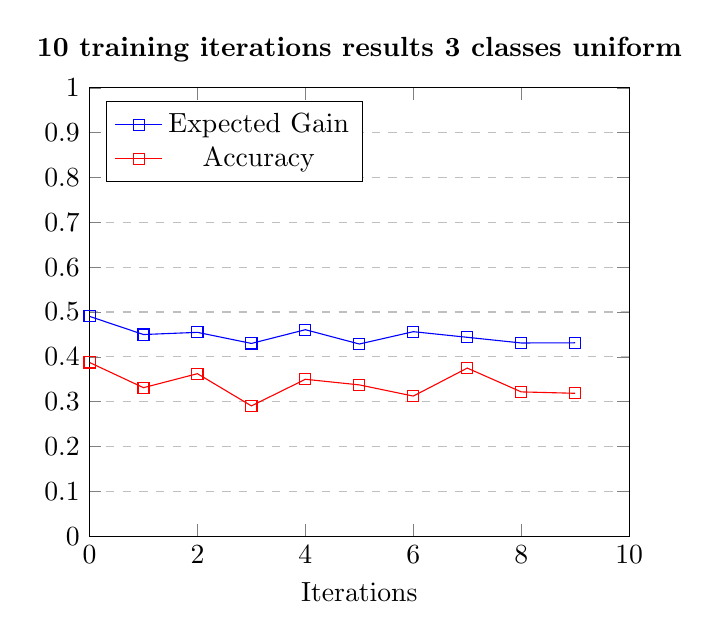
\begin{tikzpicture}
\begin{axis}[
    title=\textbf{10 training iterations results 3 classes uniform},
    xlabel={Iterations},
    xmin=0, xmax=10,
    ymin=0.0, ymax=1,
    xtick={0,2,4,6,8,10},
    ytick={0.0,0.1,0.2,0.3,0.4,0.5,0.6,0.7,0.8,0.9,1.0},
    legend pos=north west,
    ymajorgrids=true,
    grid style=dashed,
]

\addplot[color=blue, mark=square]
  coordinates {
    (0,0.49030720940283623)
    (1,0.44981632400021265)
    (2,0.4547041815965567)
    (3,0.42997913323401304)
    (4,0.46058465918279856)
    (5,0.4286678527092858)
    (6,0.45617940847773764)
    (7,0.44363621005504705)
    (8,0.4309883206227871)
    (9,0.43138157298087754)
  };
  \addlegendentry{Expected Gain}

\addplot[color=red, mark=square]
  coordinates {
    (0,0.3875)
    (1,0.33125)
    (2,0.3625)
    (3,0.290625)
    (4,0.35)
    (5,0.3375)
    (6,0.3125)
    (7,0.375)
    (8,0.321875)
    (9,0.31875)
  };
  \addlegendentry{Accuracy}
    
\end{axis}
\end{tikzpicture}
\vspace{1cm}

\subsection{Class overlapping}

To understand if the accuracies shown in the previous steps are determined by the number of classes and the overlapping caused by an assignation independent from the measurements, it was added to the program the option to avoid the overlap and assign a class based on the norm of the measurement vector. This is an arbitrary assignment chosen just by the simplicity and certainty of the assignment's uniqueness.

using the new parameter

\begin{verbatim}
  bin/midterm --classes 2 --measurements 5 \
    --iterations 10 --seed 1234 \
    --no-overlap
\end{verbatim}

\vspace{1cm}
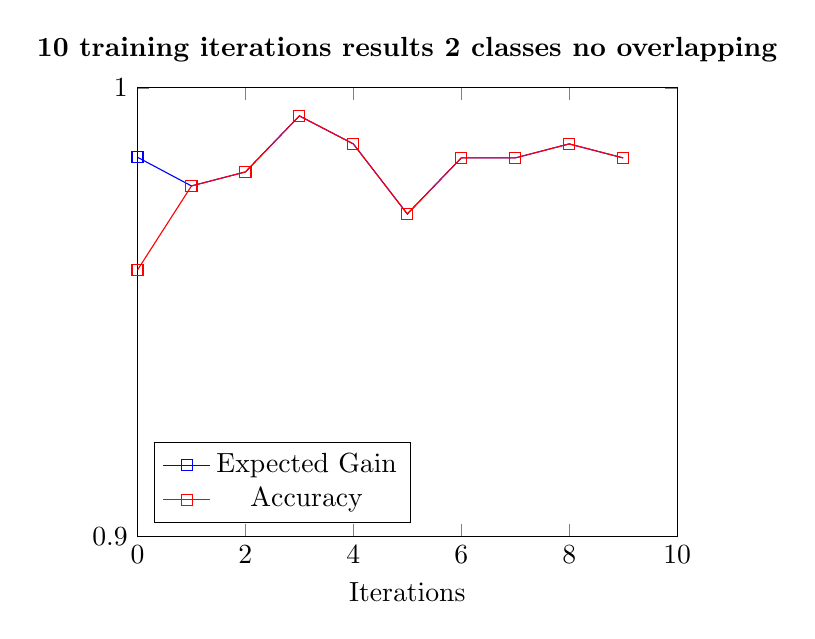
\begin{tikzpicture}
\begin{axis}[
    title=\textbf{10 training iterations results 2 classes no overlapping},
    xlabel={Iterations},
    xmin=0, xmax=10,
    ymin=0.9, ymax=1,
    xtick={0,2,4,6,8,10},
    ytick={0.9,1.0},
    legend pos=south west,
    ymajorgrids=true,
    grid style=dashed,
]

\addplot[color=blue, mark=square]
  coordinates {
    (0,0.9845253073815597)
    (1,0.9781249999999999)
    (2,0.98125)
    (3,0.9937500000000001)
    (4,0.9875000000000002)
    (5,0.971875)
    (6,0.9843750000000001)
    (7,0.9843750000000001)
    (8,0.9875000000000002)
    (9,0.9843750000000001)
  };
  \addlegendentry{Expected Gain}

\addplot[color=red, mark=square]
  coordinates {
    (0,0.959375)
    (1,0.978125)
    (2,0.98125)
    (3,0.99375)
    (4,0.9875)
    (5,0.971875)
    (6,0.984375)
    (7,0.984375)
    (8,0.9875)
    (9,0.984375)
  };
  \addlegendentry{Accuracy}
    
\end{axis}
\end{tikzpicture}
\vspace{1cm}

Now the expected gain is considerably higher, and trying with 100 iterations stays close to 1.0.

\vspace{1cm}
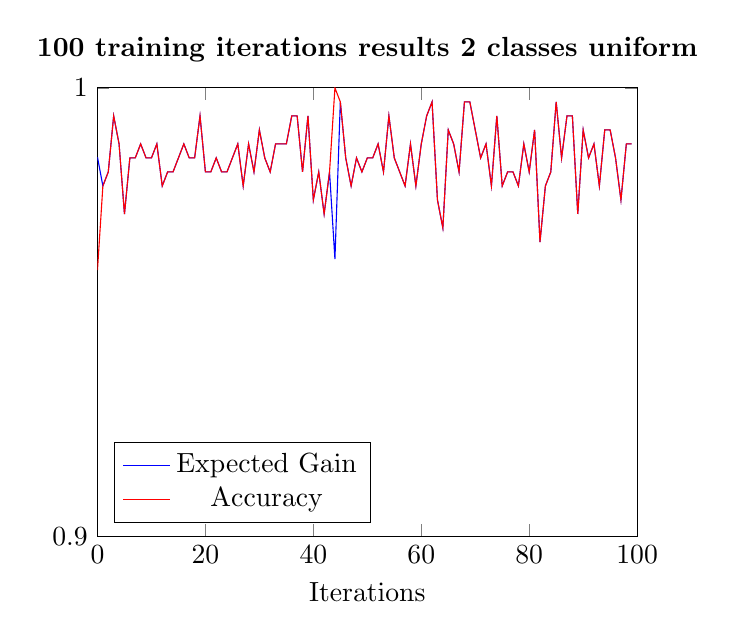
\begin{tikzpicture}
\begin{axis}[
    title=\textbf{100 training iterations results 2 classes uniform},
    xlabel={Iterations},
    xmin=0, xmax=100,
    ymin=0.9, ymax=1,
    xtick={0,20,40,60,80,100},
    ytick={0.9,1.0},
    legend pos=south west,
    ymajorgrids=true,
    grid style=dashed,
]

\addplot[color=blue, mark=dot]
  coordinates {
    (0,0.9845253073815597)
    (1,0.9781249999999999)
    (2,0.98125)
    (3,0.9937500000000001)
    (4,0.9875000000000002)
    (5,0.971875)
    (6,0.9843750000000001)
    (7,0.9843750000000001)
    (8,0.9875000000000002)
    (9,0.9843750000000001)
    (10,0.9843750000000001)
    (11,0.9875000000000002)
    (12,0.9781250000000001)
    (13,0.98125)
    (14,0.98125)
    (15,0.9843750000000001)
    (16,0.9875000000000002)
    (17,0.9843750000000001)
    (18,0.9843750000000001)
    (19,0.9937500000000001)
    (20,0.98125)
    (21,0.98125)
    (22,0.9843750000000001)
    (23,0.98125)
    (24,0.98125)
    (25,0.9843750000000001)
    (26,0.9875000000000002)
    (27,0.9781250000000001)
    (28,0.9875000000000002)
    (29,0.98125)
    (30,0.9906250000000001)
    (31,0.9843750000000001)
    (32,0.98125)
    (33,0.9875000000000002)
    (34,0.9875000000000002)
    (35,0.9875000000000002)
    (36,0.9937500000000001)
    (37,0.9937500000000001)
    (38,0.98125)
    (39,0.9937500000000001)
    (40,0.975)
    (41,0.98125)
    (42,0.971875)
    (43,0.98125)
    (44,0.9618008249288758)
    (45,0.9968750000000001)
    (46,0.9843750000000001)
    (47,0.9781250000000001)
    (48,0.9843750000000001)
    (49,0.98125)
    (50,0.9843750000000001)
    (51,0.9843750000000001)
    (52,0.9875000000000002)
    (53,0.98125)
    (54,0.9937500000000001)
    (55,0.9843750000000001)
    (56,0.98125)
    (57,0.9781250000000001)
    (58,0.9875000000000002)
    (59,0.9781250000000001)
    (60,0.9875000000000002)
    (61,0.9937500000000001)
    (62,0.9968750000000001)
    (63,0.975)
    (64,0.96875)
    (65,0.9906250000000001)
    (66,0.9875000000000002)
    (67,0.98125)
    (68,0.9968750000000001)
    (69,0.9968750000000001)
    (70,0.9906250000000001)
    (71,0.9843750000000001)
    (72,0.9875000000000002)
    (73,0.9781250000000001)
    (74,0.9937500000000001)
    (75,0.9781250000000001)
    (76,0.98125)
    (77,0.98125)
    (78,0.9781250000000001)
    (79,0.9875000000000002)
    (80,0.98125)
    (81,0.9906250000000001)
    (82,0.965625)
    (83,0.9781250000000001)
    (84,0.98125)
    (85,0.9968750000000001)
    (86,0.9843750000000001)
    (87,0.9937500000000001)
    (88,0.9937500000000001)
    (89,0.971875)
    (90,0.9906250000000001)
    (91,0.9843750000000001)
    (92,0.9875000000000002)
    (93,0.9781250000000001)
    (94,0.9906250000000001)
    (95,0.9906250000000001)
    (96,0.9843750000000001)
    (97,0.975)
    (98,0.9875000000000002)
    (99,0.9875000000000002)
  };
  \addlegendentry{Expected Gain}

\addplot[color=red]
  coordinates {
    (0,0.959375)
    (1,0.978125)
    (2,0.98125)
    (3,0.99375)
    (4,0.9875)
    (5,0.971875)
    (6,0.984375)
    (7,0.984375)
    (8,0.9875)
    (9,0.984375)
    (10,0.984375)
    (11,0.9875)
    (12,0.978125)
    (13,0.98125)
    (14,0.98125)
    (15,0.984375)
    (16,0.9875)
    (17,0.984375)
    (18,0.984375)
    (19,0.99375)
    (20,0.98125)
    (21,0.98125)
    (22,0.984375)
    (23,0.98125)
    (24,0.98125)
    (25,0.984375)
    (26,0.9875)
    (27,0.978125)
    (28,0.9875)
    (29,0.98125)
    (30,0.990625)
    (31,0.984375)
    (32,0.98125)
    (33,0.9875)
    (34,0.9875)
    (35,0.9875)
    (36,0.99375)
    (37,0.99375)
    (38,0.98125)
    (39,0.99375)
    (40,0.975)
    (41,0.98125)
    (42,0.971875)
    (43,0.98125)
    (44,1.0)
    (45,0.996875)
    (46,0.984375)
    (47,0.978125)
    (48,0.984375)
    (49,0.98125)
    (50,0.984375)
    (51,0.984375)
    (52,0.9875)
    (53,0.98125)
    (54,0.99375)
    (55,0.984375)
    (56,0.98125)
    (57,0.978125)
    (58,0.9875)
    (59,0.978125)
    (60,0.9875)
    (61,0.99375)
    (62,0.996875)
    (63,0.975)
    (64,0.96875)
    (65,0.990625)
    (66,0.9875)
    (67,0.98125)
    (68,0.996875)
    (69,0.996875)
    (70,0.990625)
    (71,0.984375)
    (72,0.9875)
    (73,0.978125)
    (74,0.99375)
    (75,0.978125)
    (76,0.98125)
    (77,0.98125)
    (78,0.978125)
    (79,0.9875)
    (80,0.98125)
    (81,0.990625)
    (82,0.965625)
    (83,0.978125)
    (84,0.98125)
    (85,0.996875)
    (86,0.984375)
    (87,0.99375)
    (88,0.99375)
    (89,0.971875)
    (90,0.990625)
    (91,0.984375)
    (92,0.9875)
    (93,0.978125)
    (94,0.990625)
    (95,0.990625)
    (96,0.984375)
    (97,0.975)
    (98,0.9875)
    (99,0.9875)
  };
  \addlegendentry{Accuracy}
    
\end{axis}
\end{tikzpicture}
\vspace{1cm}

\section{Conclusions}

This report shows a Bayes classifier written from scratch in Ruby without any scientific library, following the theory and instructions provided during the Machine Learning class.

The program includes definitions and abstractions for Dimension, Space, and DataSet that can be configured with optional parameters through the command line to create classes, measurement, and training sets.

The initial results were not the one expected, showing low and bouncing expected gains and accuracy. As a way to explain these behaviors, two paths were developed

\begin{itemize}
  \item First, create the dimensions for classes and measurements using uniform probability distribution functions, expecting more recognizable numbers. The method worked, and it allowed us to determine that the accuracy was inversely proportional to the classes' cardinality.
  \item Then, with the conclusion from the previous step, it was introduced an option to assign a class to a specific measurement without overlapping. The norm of the measurement vector was the method used, and it produced a considerable impact on the expected gain and accuracy, reaching values over $0.99$ in both parameters.
\end{itemize}

Although some aspects of the value could have been explained with the overlapping of classes, it remains inconclusive why the expected gain and accuracy are not reaching 1.0 or why it does not stop bouncing.

\begin{thebibliography}{2}

\bibitem{discrete-bayes}
Robert M. Haralick,
\textit{Discrete Bayes Pattern Recognition}
\\\texttt{\url{http://haralick.org/ML/discrete_bayes.pdf}}

\bibitem{midterm-project}
Robert M. Haralick,
\textit{Midterm Project}
\\\texttt{\url{http://haralick.org/ML/midterm_project.pdf}}

\end{thebibliography}

\end{document}
  